\documentclass[border=3pt,tikz]{standalone}
\usepackage{amsmath}
\usetikzlibrary {3d} 
\usetikzlibrary {arrows}
\usetikzlibrary{shapes.geometric}

\usetikzlibrary {3d} 
\usetikzlibrary {arrows}
\usetikzlibrary{shapes.geometric}
\begin{document}
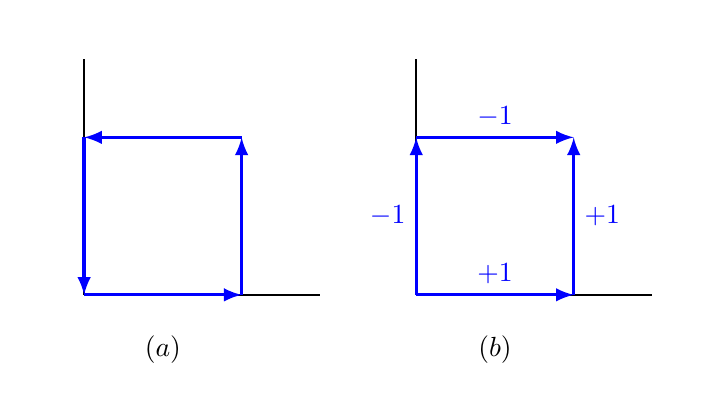
\begin{tikzpicture}[scale=2, rotate=0]
    \node[below] at(-0.3, -0.2) {};
    \node[below] at(0.3, 1.7) {};
    \draw[thick] (0.,0) -- (0, 1.5);
    \draw[thick] (0.,0) -- (1.5, 0);
    \draw [blue, -latex, very thick] (0,0) -- (1, 0);
    \draw [blue, -latex, very thick] (1,0) -- (1, 1);
    \draw [blue, -latex, very thick] (1,1) -- (0, 1);
    \draw [blue, -latex, very thick] (0,1) -- (0, 0);
    \node[below] at(0.5, -0.2) {$(a)$};
    \begin{scope}[xshift=60]
    \draw[thick] (0.,0) -- (0, 1.5);
    \draw[thick] (0.,0) -- (1.5, 0);
    \draw [blue, -latex, very thick] (0,0) -- node [above] {$+1$} (1, 0);
    \draw [blue, -latex, very thick] (1,0) -- node [right] {$+1$} (1, 1);
    \draw [blue, -latex, very thick] (0,1) -- node [above] {$-1$} (1, 1);
    \draw [blue, -latex, very thick] (0,0) -- node [left] {$-1$} (0, 1);
    \node[below] at(0.5, -0.2) {$(b)$};
    \node[below] at(1.7, 1.7) {};
    \end{scope}
  \end{tikzpicture}
\end{document}